\documentclass[twoside]{book}

% Packages required by doxygen
\usepackage{fixltx2e}
\usepackage{calc}
\usepackage{doxygen}
\usepackage[export]{adjustbox} % also loads graphicx
\usepackage{graphicx}
\usepackage[utf8]{inputenc}
\usepackage{makeidx}
\usepackage{multicol}
\usepackage{multirow}
\PassOptionsToPackage{warn}{textcomp}
\usepackage{textcomp}
\usepackage[nointegrals]{wasysym}
\usepackage[table]{xcolor}

% Font selection
\usepackage[T1]{fontenc}
\usepackage[scaled=.90]{helvet}
\usepackage{courier}
\usepackage{amssymb}
\usepackage{sectsty}
\renewcommand{\familydefault}{\sfdefault}
\allsectionsfont{%
  \fontseries{bc}\selectfont%
  \color{darkgray}%
}
\renewcommand{\DoxyLabelFont}{%
  \fontseries{bc}\selectfont%
  \color{darkgray}%
}
\newcommand{\+}{\discretionary{\mbox{\scriptsize$\hookleftarrow$}}{}{}}

% Page & text layout
\usepackage{geometry}
\geometry{%
  a4paper,%
  top=2.5cm,%
  bottom=2.5cm,%
  left=2.5cm,%
  right=2.5cm%
}
\tolerance=750
\hfuzz=15pt
\hbadness=750
\setlength{\emergencystretch}{15pt}
\setlength{\parindent}{0cm}
\setlength{\parskip}{3ex plus 2ex minus 2ex}
\makeatletter
\renewcommand{\paragraph}{%
  \@startsection{paragraph}{4}{0ex}{-1.0ex}{1.0ex}{%
    \normalfont\normalsize\bfseries\SS@parafont%
  }%
}
\renewcommand{\subparagraph}{%
  \@startsection{subparagraph}{5}{0ex}{-1.0ex}{1.0ex}{%
    \normalfont\normalsize\bfseries\SS@subparafont%
  }%
}
\makeatother

% Headers & footers
\usepackage{fancyhdr}
\pagestyle{fancyplain}
\fancyhead[LE]{\fancyplain{}{\bfseries\thepage}}
\fancyhead[CE]{\fancyplain{}{}}
\fancyhead[RE]{\fancyplain{}{\bfseries\leftmark}}
\fancyhead[LO]{\fancyplain{}{\bfseries\rightmark}}
\fancyhead[CO]{\fancyplain{}{}}
\fancyhead[RO]{\fancyplain{}{\bfseries\thepage}}
\fancyfoot[LE]{\fancyplain{}{}}
\fancyfoot[CE]{\fancyplain{}{}}
\fancyfoot[RE]{\fancyplain{}{\bfseries\scriptsize Generated by Doxygen }}
\fancyfoot[LO]{\fancyplain{}{\bfseries\scriptsize Generated by Doxygen }}
\fancyfoot[CO]{\fancyplain{}{}}
\fancyfoot[RO]{\fancyplain{}{}}
\renewcommand{\footrulewidth}{0.4pt}
\renewcommand{\chaptermark}[1]{%
  \markboth{#1}{}%
}
\renewcommand{\sectionmark}[1]{%
  \markright{\thesection\ #1}%
}

% Indices & bibliography
\usepackage{natbib}
\usepackage[titles]{tocloft}
\setcounter{tocdepth}{3}
\setcounter{secnumdepth}{5}
\makeindex

% Hyperlinks (required, but should be loaded last)
\usepackage{ifpdf}
\ifpdf
  \usepackage[pdftex,pagebackref=true]{hyperref}
\else
  \usepackage[ps2pdf,pagebackref=true]{hyperref}
\fi
\hypersetup{%
  colorlinks=true,%
  linkcolor=blue,%
  citecolor=blue,%
  unicode%
}

% Custom commands
\newcommand{\clearemptydoublepage}{%
  \newpage{\pagestyle{empty}\cleardoublepage}%
}

\usepackage{caption}
\captionsetup{labelsep=space,justification=centering,font={bf},singlelinecheck=off,skip=4pt,position=top}

%===== C O N T E N T S =====

\begin{document}

% Titlepage & ToC
\hypersetup{pageanchor=false,
             bookmarksnumbered=true,
             pdfencoding=unicode
            }
\pagenumbering{alph}
\begin{titlepage}
\vspace*{7cm}
\begin{center}%
{\Large My Project }\\
\vspace*{1cm}
{\large Generated by Doxygen 1.8.12}\\
\end{center}
\end{titlepage}
\clearemptydoublepage
\pagenumbering{roman}
\tableofcontents
\clearemptydoublepage
\pagenumbering{arabic}
\hypersetup{pageanchor=true}

%--- Begin generated contents ---
\chapter{Hierarchical Index}
\section{Class Hierarchy}
This inheritance list is sorted roughly, but not completely, alphabetically\+:\begin{DoxyCompactList}
\item \contentsline{section}{Game\+Asset}{\pageref{classGameAsset}}{}
\begin{DoxyCompactList}
\item \contentsline{section}{Cube\+Asset}{\pageref{classCubeAsset}}{}
\item \contentsline{section}{Diamond\+Asset}{\pageref{classDiamondAsset}}{}
\end{DoxyCompactList}
\item \contentsline{section}{Game\+Asset\+Manager}{\pageref{classGameAssetManager}}{}
\item \contentsline{section}{Game\+World}{\pageref{classGameWorld}}{}
\item \contentsline{section}{S\+D\+L\+Window\+Deleter}{\pageref{structSDLWindowDeleter}}{}
\end{DoxyCompactList}

\chapter{Class Index}
\section{Class List}
Here are the classes, structs, unions and interfaces with brief descriptions\+:\begin{DoxyCompactList}
\item\contentsline{section}{\hyperlink{classCubeAsset}{Cube\+Asset} }{\pageref{classCubeAsset}}{}
\item\contentsline{section}{\hyperlink{classDiamondAsset}{Diamond\+Asset} }{\pageref{classDiamondAsset}}{}
\item\contentsline{section}{\hyperlink{classFloorAsset}{Floor\+Asset} }{\pageref{classFloorAsset}}{}
\item\contentsline{section}{\hyperlink{classGameAsset}{Game\+Asset} }{\pageref{classGameAsset}}{}
\item\contentsline{section}{\hyperlink{classGameAssetManager}{Game\+Asset\+Manager} }{\pageref{classGameAssetManager}}{}
\item\contentsline{section}{\hyperlink{classGameWorld}{Game\+World} }{\pageref{classGameWorld}}{}
\item\contentsline{section}{\hyperlink{classPlacedCubeAsset}{Placed\+Cube\+Asset} }{\pageref{classPlacedCubeAsset}}{}
\item\contentsline{section}{\hyperlink{structSDLWindowDeleter}{S\+D\+L\+Window\+Deleter} }{\pageref{structSDLWindowDeleter}}{}
\end{DoxyCompactList}

\chapter{Class Documentation}
\hypertarget{classCubeAsset}{}\section{Cube\+Asset Class Reference}
\label{classCubeAsset}\index{Cube\+Asset@{Cube\+Asset}}
Inheritance diagram for Cube\+Asset\+:\begin{figure}[H]
\begin{center}
\leavevmode
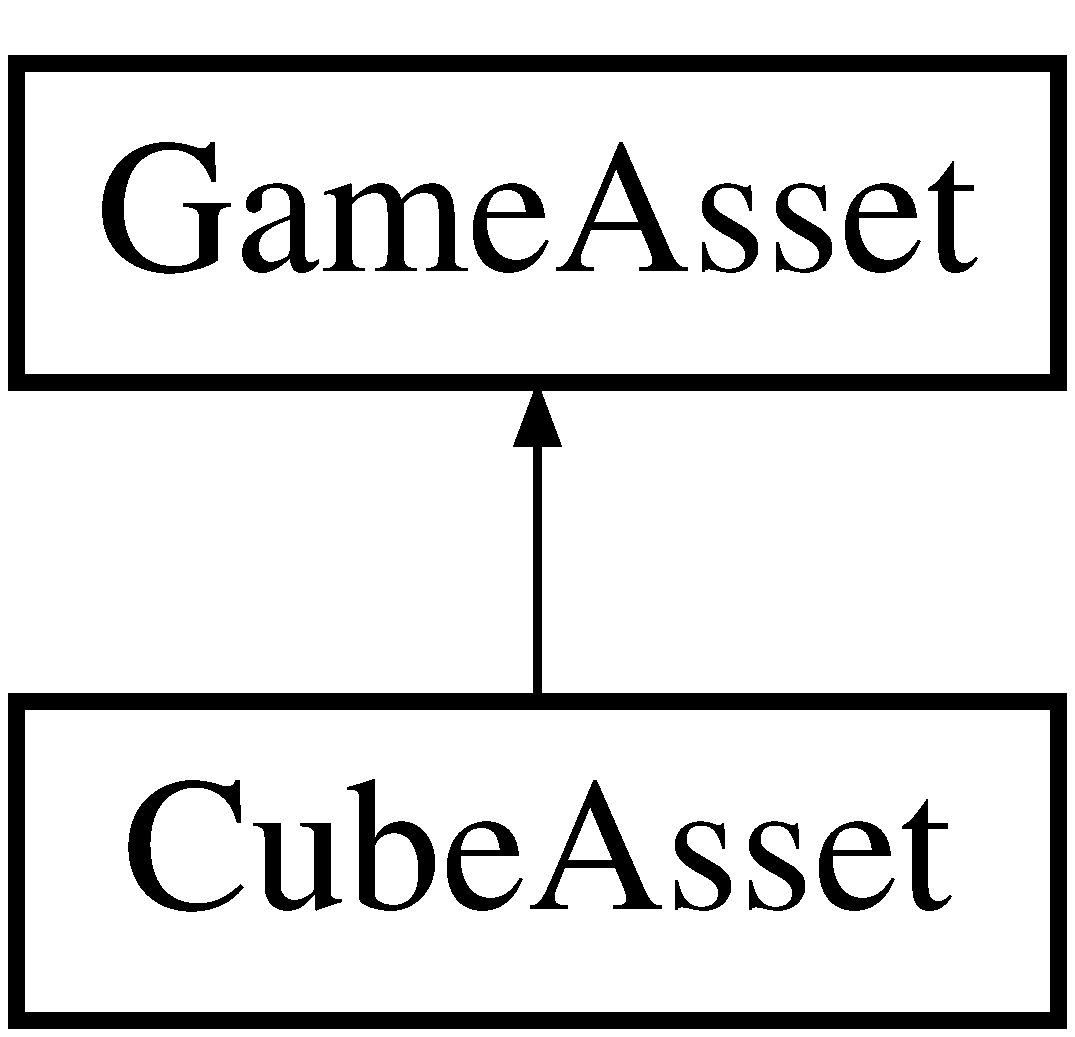
\includegraphics[height=2.000000cm]{classCubeAsset}
\end{center}
\end{figure}
\subsection*{Public Member Functions}
\begin{DoxyCompactItemize}
\item 
\hyperlink{classCubeAsset_a94f08a414e5b04ad37acffa3c1a1259b}{Cube\+Asset} (glm\+::vec3, glm\+::vec3)
\item 
virtual glm\+::vec3 \hyperlink{classCubeAsset_aacc0560317adde4d1e24eb1478790749}{get\+Pos} ()
\item 
virtual void \hyperlink{classCubeAsset_a1af568486056e254ffcf98fd99947bfe}{Draw} (G\+Luint)
\end{DoxyCompactItemize}


\subsection{Constructor \& Destructor Documentation}
\index{Cube\+Asset@{Cube\+Asset}!Cube\+Asset@{Cube\+Asset}}
\index{Cube\+Asset@{Cube\+Asset}!Cube\+Asset@{Cube\+Asset}}
\subsubsection[{\texorpdfstring{Cube\+Asset(glm\+::vec3, glm\+::vec3)}{CubeAsset(glm::vec3, glm::vec3)}}]{\setlength{\rightskip}{0pt plus 5cm}Cube\+Asset\+::\+Cube\+Asset (
\begin{DoxyParamCaption}
\item[{glm\+::vec3}]{p, }
\item[{glm\+::vec3}]{c}
\end{DoxyParamCaption}
)}\hypertarget{classCubeAsset_a94f08a414e5b04ad37acffa3c1a1259b}{}\label{classCubeAsset_a94f08a414e5b04ad37acffa3c1a1259b}
Draw cubes based on location of vertices relative to 0, assign colour based on R\+GB 

\subsection{Member Function Documentation}
\index{Cube\+Asset@{Cube\+Asset}!Draw@{Draw}}
\index{Draw@{Draw}!Cube\+Asset@{Cube\+Asset}}
\subsubsection[{\texorpdfstring{Draw(\+G\+Luint)}{Draw(GLuint)}}]{\setlength{\rightskip}{0pt plus 5cm}void Cube\+Asset\+::\+Draw (
\begin{DoxyParamCaption}
\item[{G\+Luint}]{program\+\_\+token}
\end{DoxyParamCaption}
)\hspace{0.3cm}{\ttfamily [virtual]}}\hypertarget{classCubeAsset_a1af568486056e254ffcf98fd99947bfe}{}\label{classCubeAsset_a1af568486056e254ffcf98fd99947bfe}
check for error in drawing cube 

Implements \hyperlink{classGameAsset}{Game\+Asset}.

\index{Cube\+Asset@{Cube\+Asset}!get\+Pos@{get\+Pos}}
\index{get\+Pos@{get\+Pos}!Cube\+Asset@{Cube\+Asset}}
\subsubsection[{\texorpdfstring{get\+Pos()}{getPos()}}]{\setlength{\rightskip}{0pt plus 5cm}glm\+::vec3 Cube\+Asset\+::get\+Pos (
\begin{DoxyParamCaption}
{}
\end{DoxyParamCaption}
)\hspace{0.3cm}{\ttfamily [virtual]}}\hypertarget{classCubeAsset_aacc0560317adde4d1e24eb1478790749}{}\label{classCubeAsset_aacc0560317adde4d1e24eb1478790749}
return position of cube 

Implements \hyperlink{classGameAsset}{Game\+Asset}.



The documentation for this class was generated from the following files\+:\begin{DoxyCompactItemize}
\item 
Cube\+Asset.\+h\item 
Cube\+Asset.\+cc\end{DoxyCompactItemize}

\hypertarget{classDiamondAsset}{}\section{Diamond\+Asset Class Reference}
\label{classDiamondAsset}\index{Diamond\+Asset@{Diamond\+Asset}}
Inheritance diagram for Diamond\+Asset\+:\begin{figure}[H]
\begin{center}
\leavevmode
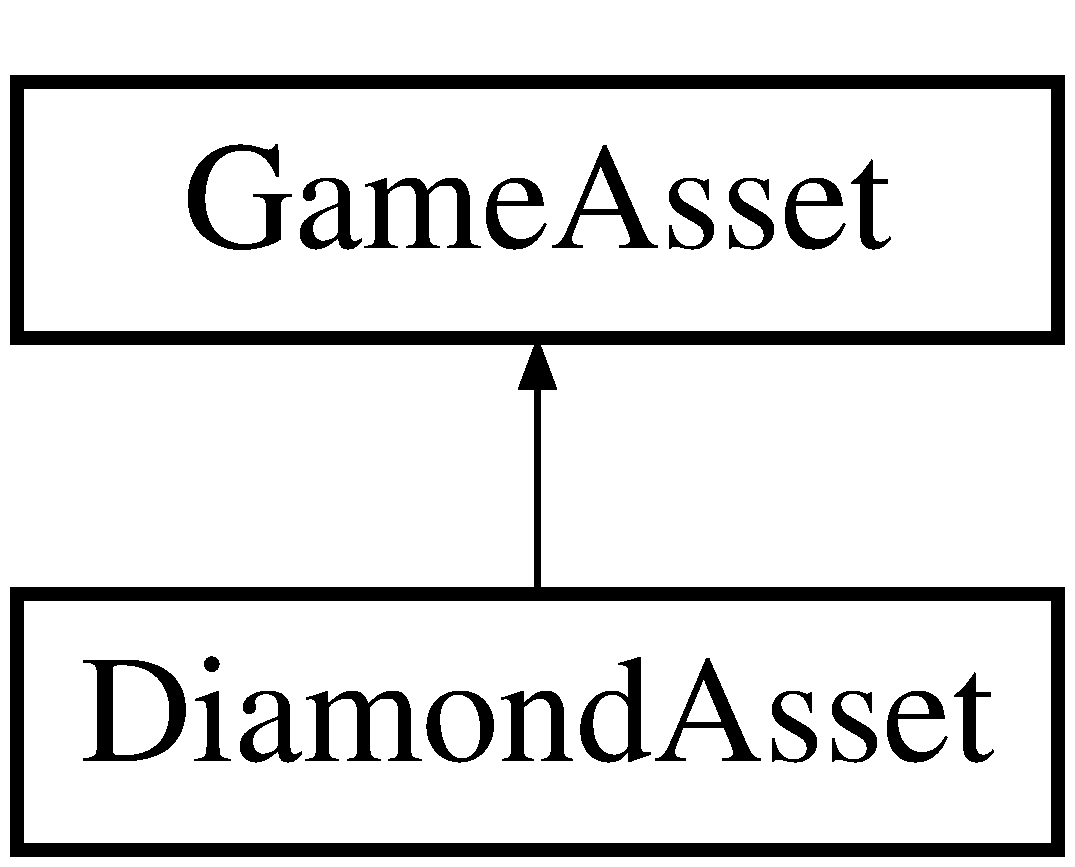
\includegraphics[height=2.000000cm]{classDiamondAsset}
\end{center}
\end{figure}
\subsection*{Public Member Functions}
\begin{DoxyCompactItemize}
\item 
\hyperlink{classDiamondAsset_af17cd961010d8b40199f8fe3b8dc1912}{Diamond\+Asset} (glm\+::vec3, glm\+::vec3)
\item 
virtual glm\+::vec3 \hyperlink{classDiamondAsset_a6821b94c4b5b6b9c5829daeed06cd86e}{get\+Pos} ()
\item 
virtual void \hyperlink{classDiamondAsset_a0c259031894623285b3b511321c73abb}{Draw} (G\+Luint)
\end{DoxyCompactItemize}


\subsection{Constructor \& Destructor Documentation}
\index{Diamond\+Asset@{Diamond\+Asset}!Diamond\+Asset@{Diamond\+Asset}}
\index{Diamond\+Asset@{Diamond\+Asset}!Diamond\+Asset@{Diamond\+Asset}}
\subsubsection[{\texorpdfstring{Diamond\+Asset(glm\+::vec3, glm\+::vec3)}{DiamondAsset(glm::vec3, glm::vec3)}}]{\setlength{\rightskip}{0pt plus 5cm}Diamond\+Asset\+::\+Diamond\+Asset (
\begin{DoxyParamCaption}
\item[{glm\+::vec3}]{p, }
\item[{glm\+::vec3}]{c}
\end{DoxyParamCaption}
)}\hypertarget{classDiamondAsset_af17cd961010d8b40199f8fe3b8dc1912}{}\label{classDiamondAsset_af17cd961010d8b40199f8fe3b8dc1912}
Draw diamond based on location of vertices relative to 0, assign colour based on R\+GB 

\subsection{Member Function Documentation}
\index{Diamond\+Asset@{Diamond\+Asset}!Draw@{Draw}}
\index{Draw@{Draw}!Diamond\+Asset@{Diamond\+Asset}}
\subsubsection[{\texorpdfstring{Draw(\+G\+Luint)}{Draw(GLuint)}}]{\setlength{\rightskip}{0pt plus 5cm}void Diamond\+Asset\+::\+Draw (
\begin{DoxyParamCaption}
\item[{G\+Luint}]{program\+\_\+token}
\end{DoxyParamCaption}
)\hspace{0.3cm}{\ttfamily [virtual]}}\hypertarget{classDiamondAsset_a0c259031894623285b3b511321c73abb}{}\label{classDiamondAsset_a0c259031894623285b3b511321c73abb}
check for error in drawing diamond 

Implements \hyperlink{classGameAsset}{Game\+Asset}.

\index{Diamond\+Asset@{Diamond\+Asset}!get\+Pos@{get\+Pos}}
\index{get\+Pos@{get\+Pos}!Diamond\+Asset@{Diamond\+Asset}}
\subsubsection[{\texorpdfstring{get\+Pos()}{getPos()}}]{\setlength{\rightskip}{0pt plus 5cm}glm\+::vec3 Diamond\+Asset\+::get\+Pos (
\begin{DoxyParamCaption}
{}
\end{DoxyParamCaption}
)\hspace{0.3cm}{\ttfamily [virtual]}}\hypertarget{classDiamondAsset_a6821b94c4b5b6b9c5829daeed06cd86e}{}\label{classDiamondAsset_a6821b94c4b5b6b9c5829daeed06cd86e}
return position of diamond 

Implements \hyperlink{classGameAsset}{Game\+Asset}.



The documentation for this class was generated from the following files\+:\begin{DoxyCompactItemize}
\item 
Diamond\+Asset.\+h\item 
Diamond\+Asset.\+cc\end{DoxyCompactItemize}

\hypertarget{classGameAsset}{}\section{Game\+Asset Class Reference}
\label{classGameAsset}\index{Game\+Asset@{Game\+Asset}}


{\ttfamily \#include $<$Game\+Asset.\+h$>$}

Inheritance diagram for Game\+Asset\+:\begin{figure}[H]
\begin{center}
\leavevmode
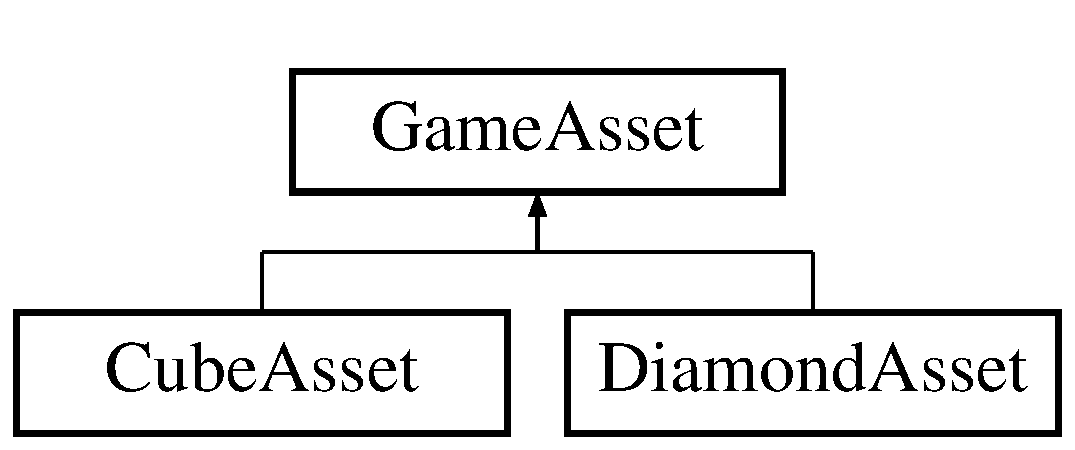
\includegraphics[height=2.000000cm]{classGameAsset}
\end{center}
\end{figure}
\subsection*{Public Member Functions}
\begin{DoxyCompactItemize}
\item 
virtual void {\bfseries Draw} (G\+Luint)=0\hypertarget{classGameAsset_a961aa51ca0a9961fc584c0b5d5431300}{}\label{classGameAsset_a961aa51ca0a9961fc584c0b5d5431300}

\item 
virtual glm\+::vec3 {\bfseries get\+Pos} ()=0\hypertarget{classGameAsset_a6b3e7c11efd7084e032f23dfd9374672}{}\label{classGameAsset_a6b3e7c11efd7084e032f23dfd9374672}

\item 
void \hyperlink{classGameAsset_af6e148d5c112bd024739ccffcbee603e}{gen\+BB} (glm\+::vec3, glm\+::vec3)
\item 
bool \hyperlink{classGameAsset_a12c7589d38ad0c59588659326e234057}{collides} (glm\+::vec3, glm\+::vec3)
\item 
bool \hyperlink{classGameAsset_a5ad5bb6e7ad41b86f3709a75ecb5bacf}{collides} (\hyperlink{classGameAsset}{Game\+Asset} \&a)
\item 
glm\+::vec3 \hyperlink{classGameAsset_a47ca91c87610d002d63f59563c038af9}{return\+Min} ()
\item 
glm\+::vec3 \hyperlink{classGameAsset_ae2661492933e0678c4c17b0f77083dc9}{return\+Max} ()
\end{DoxyCompactItemize}


\subsection{Detailed Description}
holds methods/variables which need to be access via inheritance by all asset types 

\subsection{Member Function Documentation}
\index{Game\+Asset@{Game\+Asset}!collides@{collides}}
\index{collides@{collides}!Game\+Asset@{Game\+Asset}}
\subsubsection[{\texorpdfstring{collides(glm\+::vec3, glm\+::vec3)}{collides(glm::vec3, glm::vec3)}}]{\setlength{\rightskip}{0pt plus 5cm}bool Game\+Asset\+::collides (
\begin{DoxyParamCaption}
\item[{glm\+::vec3}]{minB, }
\item[{glm\+::vec3}]{maxB}
\end{DoxyParamCaption}
)}\hypertarget{classGameAsset_a12c7589d38ad0c59588659326e234057}{}\label{classGameAsset_a12c7589d38ad0c59588659326e234057}
Check if A\+A\+B\+Bs are intersecting (passed min and max against the min and max of the current asset \index{Game\+Asset@{Game\+Asset}!collides@{collides}}
\index{collides@{collides}!Game\+Asset@{Game\+Asset}}
\subsubsection[{\texorpdfstring{collides(\+Game\+Asset \&a)}{collides(GameAsset &a)}}]{\setlength{\rightskip}{0pt plus 5cm}bool Game\+Asset\+::collides (
\begin{DoxyParamCaption}
\item[{{\bf Game\+Asset} \&}]{a}
\end{DoxyParamCaption}
)}\hypertarget{classGameAsset_a5ad5bb6e7ad41b86f3709a75ecb5bacf}{}\label{classGameAsset_a5ad5bb6e7ad41b86f3709a75ecb5bacf}
Receives a reference to an asset, calls \hyperlink{classGameAsset_a47ca91c87610d002d63f59563c038af9}{return\+Min()} and \hyperlink{classGameAsset_ae2661492933e0678c4c17b0f77083dc9}{return\+Max()} and passes these to the A\+A\+BB collision detection-\/ needed for asset-\/$>$asset collision \index{Game\+Asset@{Game\+Asset}!gen\+BB@{gen\+BB}}
\index{gen\+BB@{gen\+BB}!Game\+Asset@{Game\+Asset}}
\subsubsection[{\texorpdfstring{gen\+B\+B(glm\+::vec3, glm\+::vec3)}{genBB(glm::vec3, glm::vec3)}}]{\setlength{\rightskip}{0pt plus 5cm}void Game\+Asset\+::gen\+BB (
\begin{DoxyParamCaption}
\item[{glm\+::vec3}]{p, }
\item[{glm\+::vec3}]{param}
\end{DoxyParamCaption}
)}\hypertarget{classGameAsset_af6e148d5c112bd024739ccffcbee603e}{}\label{classGameAsset_af6e148d5c112bd024739ccffcbee603e}
generate min and max coords for A\+A\+B\+Bs \index{Game\+Asset@{Game\+Asset}!return\+Max@{return\+Max}}
\index{return\+Max@{return\+Max}!Game\+Asset@{Game\+Asset}}
\subsubsection[{\texorpdfstring{return\+Max()}{returnMax()}}]{\setlength{\rightskip}{0pt plus 5cm}glm\+::vec3 Game\+Asset\+::return\+Max (
\begin{DoxyParamCaption}
{}
\end{DoxyParamCaption}
)}\hypertarget{classGameAsset_ae2661492933e0678c4c17b0f77083dc9}{}\label{classGameAsset_ae2661492933e0678c4c17b0f77083dc9}
returns the max coordinate vector of an asset \index{Game\+Asset@{Game\+Asset}!return\+Min@{return\+Min}}
\index{return\+Min@{return\+Min}!Game\+Asset@{Game\+Asset}}
\subsubsection[{\texorpdfstring{return\+Min()}{returnMin()}}]{\setlength{\rightskip}{0pt plus 5cm}glm\+::vec3 Game\+Asset\+::return\+Min (
\begin{DoxyParamCaption}
{}
\end{DoxyParamCaption}
)}\hypertarget{classGameAsset_a47ca91c87610d002d63f59563c038af9}{}\label{classGameAsset_a47ca91c87610d002d63f59563c038af9}
returns the min coordinate vector of an asset 

The documentation for this class was generated from the following files\+:\begin{DoxyCompactItemize}
\item 
Game\+Asset.\+h\item 
Game\+Asset.\+cc\end{DoxyCompactItemize}

\hypertarget{classGameAssetManager}{}\section{Game\+Asset\+Manager Class Reference}
\label{classGameAssetManager}\index{Game\+Asset\+Manager@{Game\+Asset\+Manager}}


{\ttfamily \#include $<$Game\+Asset\+Manager.\+h$>$}

\subsection*{Public Member Functions}
\begin{DoxyCompactItemize}
\item 
\hyperlink{classGameAssetManager_aaa0d58e276cc10ad91a7457085598a71}{Game\+Asset\+Manager} (Application\+Mode)
\item 
virtual \hyperlink{classGameAssetManager_a1270bd61ecbcca563f079803e40c9b77}{$\sim$\+Game\+Asset\+Manager} ()
\item 
\hyperlink{classGameAssetManager_a2c9adcb72faa154c87eadc9bafe5269d}{Game\+Asset\+Manager} (\hyperlink{classGameAssetManager}{Game\+Asset\+Manager} const \&)
\item 
\hyperlink{classGameAssetManager_a44f6e2fd6b8ff1dd64e5697f1be7386d}{Game\+Asset\+Manager} (\hyperlink{classGameAssetManager}{Game\+Asset\+Manager} const \&\&)
\item 
void \hyperlink{classGameAssetManager_ac72678a4ad5378c685aa6bae84a4e712}{operator=} (\hyperlink{classGameAssetManager}{Game\+Asset\+Manager} const \&)
\item 
void \hyperlink{classGameAssetManager_ad3de8ff00d55ba04728b1de8213b2349}{Add\+Asset} (std\+::shared\+\_\+ptr$<$ \hyperlink{classGameAsset}{Game\+Asset} $>$)
\item 
void \hyperlink{classGameAssetManager_a32837132bd70a9a9ed537323c2d3d886}{Draw} ()
\item 
bool \hyperlink{classGameAssetManager_a72a6dcaaa2a17318df017467a2184b53}{check\+Collision} (glm\+::vec3 position)
\item 
G\+Luint \hyperlink{classGameAssetManager_a80bf9227a397b4aa416388ef94352e29}{return\+Program\+\_\+token} ()
\end{DoxyCompactItemize}


\subsection{Detailed Description}
\hyperlink{classGameAssetManager}{Game\+Asset\+Manager} is a container for Game\+Assets. It also provides utility functions to to create a simple Open\+GL program that can be used to draw a simple \hyperlink{classGameAsset}{Game\+Asset}. 

\subsection{Constructor \& Destructor Documentation}
\index{Game\+Asset\+Manager@{Game\+Asset\+Manager}!Game\+Asset\+Manager@{Game\+Asset\+Manager}}
\index{Game\+Asset\+Manager@{Game\+Asset\+Manager}!Game\+Asset\+Manager@{Game\+Asset\+Manager}}
\subsubsection[{\texorpdfstring{Game\+Asset\+Manager(\+Application\+Mode)}{GameAssetManager(ApplicationMode)}}]{\setlength{\rightskip}{0pt plus 5cm}Game\+Asset\+Manager\+::\+Game\+Asset\+Manager (
\begin{DoxyParamCaption}
\item[{Application\+Mode}]{mode}
\end{DoxyParamCaption}
)\hspace{0.3cm}{\ttfamily [explicit]}}\hypertarget{classGameAssetManager_aaa0d58e276cc10ad91a7457085598a71}{}\label{classGameAssetManager_aaa0d58e276cc10ad91a7457085598a71}
Creates a \hyperlink{classGameAssetManager}{Game\+Asset\+Manager} to load the correct shaders based on the Application\+Mode. \index{Game\+Asset\+Manager@{Game\+Asset\+Manager}!````~Game\+Asset\+Manager@{$\sim$\+Game\+Asset\+Manager}}
\index{````~Game\+Asset\+Manager@{$\sim$\+Game\+Asset\+Manager}!Game\+Asset\+Manager@{Game\+Asset\+Manager}}
\subsubsection[{\texorpdfstring{$\sim$\+Game\+Asset\+Manager()}{~GameAssetManager()}}]{\setlength{\rightskip}{0pt plus 5cm}Game\+Asset\+Manager\+::$\sim$\+Game\+Asset\+Manager (
\begin{DoxyParamCaption}
{}
\end{DoxyParamCaption}
)\hspace{0.3cm}{\ttfamily [virtual]}}\hypertarget{classGameAssetManager_a1270bd61ecbcca563f079803e40c9b77}{}\label{classGameAssetManager_a1270bd61ecbcca563f079803e40c9b77}
Deletes a \hyperlink{classGameAssetManager}{Game\+Asset\+Manager}, in particular it will clean up any modifications to the Open\+GL state. \index{Game\+Asset\+Manager@{Game\+Asset\+Manager}!Game\+Asset\+Manager@{Game\+Asset\+Manager}}
\index{Game\+Asset\+Manager@{Game\+Asset\+Manager}!Game\+Asset\+Manager@{Game\+Asset\+Manager}}
\subsubsection[{\texorpdfstring{Game\+Asset\+Manager(\+Game\+Asset\+Manager const \&)}{GameAssetManager(GameAssetManager const &)}}]{\setlength{\rightskip}{0pt plus 5cm}Game\+Asset\+Manager\+::\+Game\+Asset\+Manager (
\begin{DoxyParamCaption}
\item[{{\bf Game\+Asset\+Manager} const \&}]{the\+\_\+manager}
\end{DoxyParamCaption}
)}\hypertarget{classGameAssetManager_a2c9adcb72faa154c87eadc9bafe5269d}{}\label{classGameAssetManager_a2c9adcb72faa154c87eadc9bafe5269d}
Unimplemented copy constructor -- this means that the \hyperlink{classGameAssetManager}{Game\+Asset\+Manager} may not work as you\textquotesingle{}d expect when being copied. \index{Game\+Asset\+Manager@{Game\+Asset\+Manager}!Game\+Asset\+Manager@{Game\+Asset\+Manager}}
\index{Game\+Asset\+Manager@{Game\+Asset\+Manager}!Game\+Asset\+Manager@{Game\+Asset\+Manager}}
\subsubsection[{\texorpdfstring{Game\+Asset\+Manager(\+Game\+Asset\+Manager const \&\&)}{GameAssetManager(GameAssetManager const &&)}}]{\setlength{\rightskip}{0pt plus 5cm}Game\+Asset\+Manager\+::\+Game\+Asset\+Manager (
\begin{DoxyParamCaption}
\item[{{\bf Game\+Asset\+Manager} const \&\&}]{the\+\_\+manager}
\end{DoxyParamCaption}
)}\hypertarget{classGameAssetManager_a44f6e2fd6b8ff1dd64e5697f1be7386d}{}\label{classGameAssetManager_a44f6e2fd6b8ff1dd64e5697f1be7386d}
Unimplemented move constructor -- this unimplemented method violates the C++11 move semantics for \hyperlink{classGameAssetManager}{Game\+Asset\+Manager}. 

\subsection{Member Function Documentation}
\index{Game\+Asset\+Manager@{Game\+Asset\+Manager}!Add\+Asset@{Add\+Asset}}
\index{Add\+Asset@{Add\+Asset}!Game\+Asset\+Manager@{Game\+Asset\+Manager}}
\subsubsection[{\texorpdfstring{Add\+Asset(std\+::shared\+\_\+ptr$<$ Game\+Asset $>$)}{AddAsset(std::shared_ptr< GameAsset >)}}]{\setlength{\rightskip}{0pt plus 5cm}void Game\+Asset\+Manager\+::\+Add\+Asset (
\begin{DoxyParamCaption}
\item[{std\+::shared\+\_\+ptr$<$ {\bf Game\+Asset} $>$}]{the\+\_\+asset}
\end{DoxyParamCaption}
)}\hypertarget{classGameAssetManager_ad3de8ff00d55ba04728b1de8213b2349}{}\label{classGameAssetManager_ad3de8ff00d55ba04728b1de8213b2349}
Adds a \hyperlink{classGameAsset}{Game\+Asset} to the scene graph. \index{Game\+Asset\+Manager@{Game\+Asset\+Manager}!check\+Collision@{check\+Collision}}
\index{check\+Collision@{check\+Collision}!Game\+Asset\+Manager@{Game\+Asset\+Manager}}
\subsubsection[{\texorpdfstring{check\+Collision(glm\+::vec3 position)}{checkCollision(glm::vec3 position)}}]{\setlength{\rightskip}{0pt plus 5cm}bool Game\+Asset\+Manager\+::check\+Collision (
\begin{DoxyParamCaption}
\item[{glm\+::vec3}]{p}
\end{DoxyParamCaption}
)}\hypertarget{classGameAssetManager_a72a6dcaaa2a17318df017467a2184b53}{}\label{classGameAssetManager_a72a6dcaaa2a17318df017467a2184b53}
Check for collisions by looping through each item in draw list, getting position and comparing position to camera location. \index{Game\+Asset\+Manager@{Game\+Asset\+Manager}!Draw@{Draw}}
\index{Draw@{Draw}!Game\+Asset\+Manager@{Game\+Asset\+Manager}}
\subsubsection[{\texorpdfstring{Draw()}{Draw()}}]{\setlength{\rightskip}{0pt plus 5cm}void Game\+Asset\+Manager\+::\+Draw (
\begin{DoxyParamCaption}
{}
\end{DoxyParamCaption}
)}\hypertarget{classGameAssetManager_a32837132bd70a9a9ed537323c2d3d886}{}\label{classGameAssetManager_a32837132bd70a9a9ed537323c2d3d886}
Draws each \hyperlink{classGameAsset}{Game\+Asset} in the scene graph. \index{Game\+Asset\+Manager@{Game\+Asset\+Manager}!operator=@{operator=}}
\index{operator=@{operator=}!Game\+Asset\+Manager@{Game\+Asset\+Manager}}
\subsubsection[{\texorpdfstring{operator=(\+Game\+Asset\+Manager const \&)}{operator=(GameAssetManager const &)}}]{\setlength{\rightskip}{0pt plus 5cm}void Game\+Asset\+Manager\+::operator= (
\begin{DoxyParamCaption}
\item[{{\bf Game\+Asset\+Manager} const \&}]{the\+\_\+manager}
\end{DoxyParamCaption}
)}\hypertarget{classGameAssetManager_ac72678a4ad5378c685aa6bae84a4e712}{}\label{classGameAssetManager_ac72678a4ad5378c685aa6bae84a4e712}
Unimplemented assisgnment operator -- violates the expected semantics for assignment in C++11. \index{Game\+Asset\+Manager@{Game\+Asset\+Manager}!return\+Program\+\_\+token@{return\+Program\+\_\+token}}
\index{return\+Program\+\_\+token@{return\+Program\+\_\+token}!Game\+Asset\+Manager@{Game\+Asset\+Manager}}
\subsubsection[{\texorpdfstring{return\+Program\+\_\+token()}{returnProgram_token()}}]{\setlength{\rightskip}{0pt plus 5cm}G\+Luint Game\+Asset\+Manager\+::return\+Program\+\_\+token (
\begin{DoxyParamCaption}
{}
\end{DoxyParamCaption}
)}\hypertarget{classGameAssetManager_a80bf9227a397b4aa416388ef94352e29}{}\label{classGameAssetManager_a80bf9227a397b4aa416388ef94352e29}
return program token to use in gameworld 

The documentation for this class was generated from the following files\+:\begin{DoxyCompactItemize}
\item 
Game\+Asset\+Manager.\+h\item 
Game\+Asset\+Manager.\+cc\end{DoxyCompactItemize}

\hypertarget{classGameWorld}{}\section{Game\+World Class Reference}
\label{classGameWorld}\index{Game\+World@{Game\+World}}


{\ttfamily \#include $<$Game\+World.\+h$>$}

\subsection*{Public Member Functions}
\begin{DoxyCompactItemize}
\item 
\hyperlink{classGameWorld_a17a84e57a80600961088afc753036f89}{Game\+World} (Application\+Mode)
\item 
void \hyperlink{classGameWorld_a275418607d8286979b276f165ad5876b}{Draw} ()
\item 
void \hyperlink{classGameWorld_a863eb5b4a6d30e050543490b73c03351}{move\+\_\+forward} ()
\item 
void \hyperlink{classGameWorld_a0a6ee18221d04443c70a63951f098f10}{move\+\_\+back} ()
\item 
void \hyperlink{classGameWorld_a87e9cc176c5958342b54e33e76bf6227}{move\+\_\+left} ()
\item 
void \hyperlink{classGameWorld_a96063357a010c28ba7ef3ceb691fc897}{move\+\_\+right} ()
\item 
void \hyperlink{classGameWorld_a6c5708858337e5f863818760011af50f}{add\+\_\+cube} ()
\item 
void \hyperlink{classGameWorld_a0c8016380349f7087dd6ddddcce90f0b}{add\+\_\+diamond} ()
\item 
void \hyperlink{classGameWorld_a827a524c738a252fe1ab87f45fcece71}{move\+\_\+jump} (G\+Lfloat)
\item 
bool \hyperlink{classGameWorld_a9b35d52aa5239be36a480df580c517f8}{can\+Jump} ()
\item 
void \hyperlink{classGameWorld_adf31c1e081b761f1510f0f4053c7f463}{set\+\_\+camera} (G\+Lfloat, G\+Lfloat)
\end{DoxyCompactItemize}
\subsection*{Public Attributes}
\begin{DoxyCompactItemize}
\item 
int {\bfseries jumplength} = 0\hypertarget{classGameWorld_ad2297c4f2d1f8f97bd553a2d1d48a532}{}\label{classGameWorld_ad2297c4f2d1f8f97bd553a2d1d48a532}

\end{DoxyCompactItemize}


\subsection{Detailed Description}
\hyperlink{classGameWorld}{Game\+World} allows us to separate the management of the game world from the nuts and bolts of game loop initialisation. The \hyperlink{classGameWorld}{Game\+World} currently has a very simplified scene graph consisiting of a single \hyperlink{classGameAssetManager}{Game\+Asset\+Manager}. 

\subsection{Constructor \& Destructor Documentation}
\index{Game\+World@{Game\+World}!Game\+World@{Game\+World}}
\index{Game\+World@{Game\+World}!Game\+World@{Game\+World}}
\subsubsection[{\texorpdfstring{Game\+World(\+Application\+Mode)}{GameWorld(ApplicationMode)}}]{\setlength{\rightskip}{0pt plus 5cm}Game\+World\+::\+Game\+World (
\begin{DoxyParamCaption}
\item[{Application\+Mode}]{mode}
\end{DoxyParamCaption}
)}\hypertarget{classGameWorld_a17a84e57a80600961088afc753036f89}{}\label{classGameWorld_a17a84e57a80600961088afc753036f89}
We thread the Application\+Mode through the \hyperlink{classGameWorld}{Game\+World} ss we want to read it in from the user. Threading the state through the various function calls is preferable (in this case) to having some kind of global state.

Create cube and diamond assets and assign location and color 

\subsection{Member Function Documentation}
\index{Game\+World@{Game\+World}!add\+\_\+cube@{add\+\_\+cube}}
\index{add\+\_\+cube@{add\+\_\+cube}!Game\+World@{Game\+World}}
\subsubsection[{\texorpdfstring{add\+\_\+cube()}{add_cube()}}]{\setlength{\rightskip}{0pt plus 5cm}void Game\+World\+::add\+\_\+cube (
\begin{DoxyParamCaption}
{}
\end{DoxyParamCaption}
)}\hypertarget{classGameWorld_a6c5708858337e5f863818760011af50f}{}\label{classGameWorld_a6c5708858337e5f863818760011af50f}
add cube to game space from mouse input \index{Game\+World@{Game\+World}!add\+\_\+diamond@{add\+\_\+diamond}}
\index{add\+\_\+diamond@{add\+\_\+diamond}!Game\+World@{Game\+World}}
\subsubsection[{\texorpdfstring{add\+\_\+diamond()}{add_diamond()}}]{\setlength{\rightskip}{0pt plus 5cm}void Game\+World\+::add\+\_\+diamond (
\begin{DoxyParamCaption}
{}
\end{DoxyParamCaption}
)}\hypertarget{classGameWorld_a0c8016380349f7087dd6ddddcce90f0b}{}\label{classGameWorld_a0c8016380349f7087dd6ddddcce90f0b}
add diamond to game space from mouse input \index{Game\+World@{Game\+World}!can\+Jump@{can\+Jump}}
\index{can\+Jump@{can\+Jump}!Game\+World@{Game\+World}}
\subsubsection[{\texorpdfstring{can\+Jump()}{canJump()}}]{\setlength{\rightskip}{0pt plus 5cm}bool Game\+World\+::can\+Jump (
\begin{DoxyParamCaption}
{}
\end{DoxyParamCaption}
)}\hypertarget{classGameWorld_a9b35d52aa5239be36a480df580c517f8}{}\label{classGameWorld_a9b35d52aa5239be36a480df580c517f8}
checks if jumping is enabled (can only jump once between player touching solid ground) \index{Game\+World@{Game\+World}!Draw@{Draw}}
\index{Draw@{Draw}!Game\+World@{Game\+World}}
\subsubsection[{\texorpdfstring{Draw()}{Draw()}}]{\setlength{\rightskip}{0pt plus 5cm}void Game\+World\+::\+Draw (
\begin{DoxyParamCaption}
{}
\end{DoxyParamCaption}
)}\hypertarget{classGameWorld_a275418607d8286979b276f165ad5876b}{}\label{classGameWorld_a275418607d8286979b276f165ad5876b}
Calling \hyperlink{classGameWorld_a275418607d8286979b276f165ad5876b}{Draw()} will draw the entire world.

loop to draw the world and all assets and qualities \index{Game\+World@{Game\+World}!move\+\_\+back@{move\+\_\+back}}
\index{move\+\_\+back@{move\+\_\+back}!Game\+World@{Game\+World}}
\subsubsection[{\texorpdfstring{move\+\_\+back()}{move_back()}}]{\setlength{\rightskip}{0pt plus 5cm}void Game\+World\+::move\+\_\+back (
\begin{DoxyParamCaption}
{}
\end{DoxyParamCaption}
)}\hypertarget{classGameWorld_a0a6ee18221d04443c70a63951f098f10}{}\label{classGameWorld_a0a6ee18221d04443c70a63951f098f10}
keyboard input for moving back with collision detection \index{Game\+World@{Game\+World}!move\+\_\+forward@{move\+\_\+forward}}
\index{move\+\_\+forward@{move\+\_\+forward}!Game\+World@{Game\+World}}
\subsubsection[{\texorpdfstring{move\+\_\+forward()}{move_forward()}}]{\setlength{\rightskip}{0pt plus 5cm}void Game\+World\+::move\+\_\+forward (
\begin{DoxyParamCaption}
{}
\end{DoxyParamCaption}
)}\hypertarget{classGameWorld_a863eb5b4a6d30e050543490b73c03351}{}\label{classGameWorld_a863eb5b4a6d30e050543490b73c03351}
keyboard input for moving forwards with collision detection \index{Game\+World@{Game\+World}!move\+\_\+jump@{move\+\_\+jump}}
\index{move\+\_\+jump@{move\+\_\+jump}!Game\+World@{Game\+World}}
\subsubsection[{\texorpdfstring{move\+\_\+jump(\+G\+Lfloat)}{move_jump(GLfloat)}}]{\setlength{\rightskip}{0pt plus 5cm}void Game\+World\+::move\+\_\+jump (
\begin{DoxyParamCaption}
\item[{G\+Lfloat}]{speed}
\end{DoxyParamCaption}
)}\hypertarget{classGameWorld_a827a524c738a252fe1ab87f45fcece71}{}\label{classGameWorld_a827a524c738a252fe1ab87f45fcece71}
keyboard input for jump with controlled jump speed \index{Game\+World@{Game\+World}!move\+\_\+left@{move\+\_\+left}}
\index{move\+\_\+left@{move\+\_\+left}!Game\+World@{Game\+World}}
\subsubsection[{\texorpdfstring{move\+\_\+left()}{move_left()}}]{\setlength{\rightskip}{0pt plus 5cm}void Game\+World\+::move\+\_\+left (
\begin{DoxyParamCaption}
{}
\end{DoxyParamCaption}
)}\hypertarget{classGameWorld_a87e9cc176c5958342b54e33e76bf6227}{}\label{classGameWorld_a87e9cc176c5958342b54e33e76bf6227}
keyboard input for moving left with collision detection \index{Game\+World@{Game\+World}!move\+\_\+right@{move\+\_\+right}}
\index{move\+\_\+right@{move\+\_\+right}!Game\+World@{Game\+World}}
\subsubsection[{\texorpdfstring{move\+\_\+right()}{move_right()}}]{\setlength{\rightskip}{0pt plus 5cm}void Game\+World\+::move\+\_\+right (
\begin{DoxyParamCaption}
{}
\end{DoxyParamCaption}
)}\hypertarget{classGameWorld_a96063357a010c28ba7ef3ceb691fc897}{}\label{classGameWorld_a96063357a010c28ba7ef3ceb691fc897}
keyboard input for moving right with collision detection \index{Game\+World@{Game\+World}!set\+\_\+camera@{set\+\_\+camera}}
\index{set\+\_\+camera@{set\+\_\+camera}!Game\+World@{Game\+World}}
\subsubsection[{\texorpdfstring{set\+\_\+camera(\+G\+Lfloat, G\+Lfloat)}{set_camera(GLfloat, GLfloat)}}]{\setlength{\rightskip}{0pt plus 5cm}void Game\+World\+::set\+\_\+camera (
\begin{DoxyParamCaption}
\item[{G\+Lfloat}]{x, }
\item[{G\+Lfloat}]{y}
\end{DoxyParamCaption}
)}\hypertarget{classGameWorld_adf31c1e081b761f1510f0f4053c7f463}{}\label{classGameWorld_adf31c1e081b761f1510f0f4053c7f463}
fix camera to the center of the screen and limit range 

The documentation for this class was generated from the following files\+:\begin{DoxyCompactItemize}
\item 
Game\+World.\+h\item 
Game\+World.\+cc\end{DoxyCompactItemize}

\hypertarget{structSDLWindowDeleter}{}\section{S\+D\+L\+Window\+Deleter Struct Reference}
\label{structSDLWindowDeleter}\index{S\+D\+L\+Window\+Deleter@{S\+D\+L\+Window\+Deleter}}
\subsection*{Public Member Functions}
\begin{DoxyCompactItemize}
\item 
void {\bfseries operator()} (S\+D\+L\+\_\+\+Window $\ast$window)\hypertarget{structSDLWindowDeleter_a2aedcc99c3756ae090c38badabeb10b1}{}\label{structSDLWindowDeleter_a2aedcc99c3756ae090c38badabeb10b1}

\end{DoxyCompactItemize}


The documentation for this struct was generated from the following file\+:\begin{DoxyCompactItemize}
\item 
main.\+cc\end{DoxyCompactItemize}

%--- End generated contents ---

% Index
\backmatter
\newpage
\phantomsection
\clearemptydoublepage
\addcontentsline{toc}{chapter}{Index}
\printindex

\end{document}
